\documentclass{beamer}

% Copyright 2010 Drow Ltd.
% 
% In principle, this file can be redistributed and/or modified under
% the terms of the GNU Public License, version 2.
% 
% However, this file is supposed to be a template to be modified
% for your own needs. For this reason, if you use this file as a
% template and not specifically distribute it as part of a another
% package/program, I grant the extra permission to freely copy and
% modify this file as you see fit and even to delete this copyright
% notice. 
\mode<presentation>
{
  \usetheme[titleline=true,
  alternativetitlepage=true,
  titlepagelogo=images/Java_logo]{Torino}
  \usecolortheme{nouvelle}
  \beamertemplatenavigationsymbolsempty
}

\usepackage{times}
\usepackage[utf8]{inputenc}
\usepackage[english,bulgarian]{babel}
\usepackage[T2A]{fontenc}

\usepackage{listings}
\lstset{language=Java,
  captionpos=b,
  tabsize=4,
  keywordstyle=\color{blue},
  commentstyle=\color{gray},
  stringstyle=\color{green},
  numbers=left,
  breaklines=true,
  showstringspaces=false,
  basicstyle=\ttfamily,
  emph={label},
  frame=shadowbox, 
  rulesepcolor=\color{blue},
  columns=fixed}

\title{Наследяване и полиморфизъм}

\author{инж. Божидар ~Бацов}

\institute{Drow Ltd.}

\date{16.11.2010}

\subject{Talks}
% This is only inserted into the PDF information catalog. Can be left
% out. 

\begin{document}

\begin{frame}
  \titlepage
\end{frame}

\begin{frame}{Съдържание}
  \transdissolve
  \tableofcontents[pausesections]
\end{frame}

\section{Наследяване}

\begin{frame}{Модификатори за достъп}
  \transdissolve
  \begin{itemize}
    \item Ограничават видимостта на класовете и техните членове
    \item Могат да се прилагат върху класове, методи и полета
    \begin{itemize}
    \item \textcolor{blue}{private}
      \begin{itemize}
      \item достъп само в рамките на класа
      \end{itemize}
    \item \textcolor{blue}{public}
      \begin{itemize}
      \item достъп за всички
      \end{itemize}
    \item default(package)
      \begin{itemize}
      \item достъп за всички в пакета
      \end{itemize}
    \item \textcolor{blue}{protected}
      \begin{itemize}
      \item default + достъп в наследените
      \end{itemize}
    \end{itemize}    
  \end{itemize}
\end{frame}

\begin{frame}{Наследяване}
  \transdissolve
  \begin{itemize}
  \item Фундаментална техника в ООП
  \item Изграждане на нови класове върху основата на съществуващи
    класове
  \item Преизползват се методите и полетата на съществуващи класове
  \item Добавя се ново поведение и състояние
  \item Променя се съществуващото поведение
  \end{itemize}
\end{frame}

\begin{frame}{Концептуален пример}
  \transdissolve
  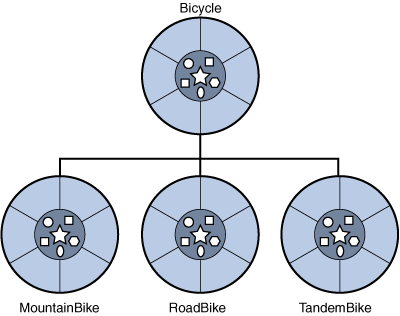
\includegraphics[width=320px, height=150px]{images/concepts-inheritance.png}  
\end{frame}

\begin{frame}{От общото към частното}
  \transdissolve
  \begin{itemize}
  \item наследяване == разширяване
  \item суперклас(клас родител/базов клас)
  \item подклас(клас наследник)
  \item отношението между подклас и суперклас е е(is-a)
    \begin{itemize}
      \item Планинското колело е колело.
      \item Програмистът е човек.
    \end{itemize}
  \end{itemize}
\end{frame}

\begin{frame}[fragile]
  \frametitle{Наследяване - синтаксис}
  \transdissolve
\begin{lstlisting}
class SubClass extends SuperClass {
  // fields
  ...
  // constructors
  ...
  // methods
  ...
}
\end{lstlisting}
\end{frame}

\begin{frame}{Ключови моменти при наследяването}
  \transdissolve
  \begin{itemize}
  \item Конструкторът на подкласа извиква конструктора на суперкласа
  \item \textcolor{blue}{private} елементите не са достъпни директно в подкласовете
  \item Ключовата дума \textcolor{blue}{super} позволява обръщение към метод от
    суперкласа
  \end{itemize}
\end{frame}

\begin{frame}{Йерархия на наследяването}
  \transdissolve
  \begin{itemize}
  \item Единична йерархия на наследяване - един подклас може да има
    само един суперклас
  \item Избягват се много от проблемите на C++
  \item Интерфейсите предлагат подобие на множествено наследяване
  \end{itemize}
\end{frame}

\begin{frame}{Диаграма}
  \transdissolve
\end{frame}

\section{Полиморфизъм}

\begin{frame}[fragile]
  \frametitle{Полиморфизъм}
  \transdissolve
  \begin{itemize}
    \item Променливи от суперклас могат да бъдат асоциирани с обекти
      от подкласове
    \item Виртуалната машина знае истинските типове на обектите и по
      време на изпълнение извиква техните методи, независимо с
      променлива от какъв тип са асоциирани
    \item Полиморфизмът е тясно свързан с късното свързване на
    методите(late binding).
  \end{itemize}
  \begin{lstlisting}
Programmer p = new Programmer();
Employee e = new Programmer();
  \end{lstlisting}
\end{frame}

\begin{frame}{Предимства на полиморфизма}
  \transdissolve
  \begin{itemize}
  \item Ниска свързаност(loose coupling)
  \item Гъвкавост
    \begin{itemize}
    \item нови класове могат да бъдат добавяни през
      прекомпилиране на кода
    \end{itemize}
  \item Простота
    \begin{itemize}
    \item придържаме ме се към по-прост интерфейс
    \end{itemize}
  \end{itemize}
\end{frame}

\begin{frame}{Търсене на метод}
  \transdissolve
  \begin{itemize}
  \item Търсене от компилатора(ранно/статично свързване)
  \item Търсене от виртуалната машина(късно/динамично свързване)
  \item Таблица на методите
  \end{itemize}
\end{frame}

\begin{frame}{Късно свързване}
  \transdissolve
  \begin{itemize}
  \item Виртуалната машина знае истинския тип на всеки един обект
  \item Виртуалната машина изпълнява методите на базата на истинския
    тип
  \item Необходимост за реализиране на полиморфизъм
  \end{itemize}
\end{frame}

\begin{frame}{Забраняване на наследяването и късното свързване}
  \transdissolve
  \begin{itemize}
  \item final class - неразширяем клас
  \item final method - метод, който не може да бъде динамично свързан
  \item Във final class всички методи са имплицитно final
  \item final като оптимизационна и защитна техника
  \end{itemize}
\end{frame}

\begin{frame}{Абстрактни класове}
  \transdissolve
  \begin{itemize}
  \item Създадени да бъдат разширявани
  \item Не могат да бъдат инстанцирани
  \item Обикновено са на върха на йерархията на наследяването
  \item Съдържат един или повече методи без имплементация(абстрактни методи)
  \end{itemize}
\end{frame}

\begin{frame}[fragile]
  \frametitle{Абстрактни класове - пример}
  \transdissolve
\begin{lstlisting}
abstract class SomeClass {
     abstract void doSomething();
}
SomeClass sc = new SomeClass(); // ERROR
\end{lstlisting}
\end{frame}

\begin{frame}[fragile]
  \frametitle{Преобразуване на обекти}
  \transdissolve
  \begin{itemize}
  \item Всеки обект от подклас и е обект от суперкласа
  \item Обратното не е вярно
  \end{itemize}
\begin{lstlisting}
Programmer p = new Programmer();
Employee e = p;
e = new Employee();
p = e;
\end{lstlisting}
\end{frame}

\begin{frame}[fragile]
  \frametitle{Преобразуване на обекти}
  \transdissolve
  \begin{itemize}
  \item Референция от суперклас може да бъде конвертирана до
    референция от подклас изрично
    \begin{lstlisting}
Employee e = new Programmer();
Programmer p = (Programmer) e;
    \end{lstlisting}
  \item Изричното преобразуване е опасна операция, която може да
    доведе го грешки по време на изпълнение на програмата
  \end{itemize}
\end{frame}

\begin{frame}[fragile]
  \frametitle{Преобразуване на обекти}
  \transdissolve
  \begin{itemize}
  \item Сигурно преобразуване с instanceof
    \begin{lstlisting}
if (e instanceof Programmer) {
  p = (Programmer) e;
}
    \end{lstlisting}
  \item Невъзможните преобразувания се улавят от компилатора
    \begin{lstlisting}
Date d = (Date) e;
    \end{lstlisting}
  \end{itemize}
\end{frame}

\begin{frame}{Върховния суперклас Object}
  \transdissolve
  \begin{itemize}
  \item Начало на класовата йерархия в Java
  \item Всеки клас имплицитно наследява Object
  \item Съдържа в себе си методи, които имат смисъл за всички обекти
    \begin{itemize}
      \item clone
      \item equals
      \item hashCode
      \item toString
    \end{itemize}
  \item Всяка референция може да бъде преобразувана до тип Object
  \end{itemize}
\end{frame}

\begin{frame}{Върховния суперклас Object}
  \transdissolve
  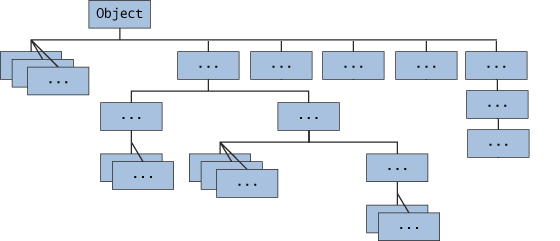
\includegraphics[width=320px, height=150px]{images/classes-object.png}
\end{frame}


\begin{frame}{Сравняване на обекти}
  \transdissolve
  \begin{itemize}
  \item == сравнява референции - сравнение за идентичност
  \item метода equals()
  \item Дефиниране на подходящ метод equals()
    \begin{itemize}
      \item проверка за сравнение с null
      \item проверка за сравнение със същия обект
      \item проверка за сравнение с различен тип
      \item сравняване на двата обекта по полета
      \begin{itemize}
        \item рекурсивно сравняване на полета от референтни типове с equals
      \end{itemize}
    \end{itemize}
  \item връзка между equals и hashCode
  \end{itemize}
\end{frame}

\begin{frame}{Модификатор за достъп protected}
  \transdissolve
  \begin{itemize}
  \item Еквивалент на default достъп + директен достъп в подкласовете
  \item Употребата му се счита за лош стил
  \item protected и default е желателно да бъдат избягвани
  \item четири нива на достъп
    \begin{itemize}
      \item private
      \item public
      \item default(package)
      \item protected
    \end{itemize}
  \item три модификатора за достъп
    \begin{itemize}
      \item private
      \item public
      \item protected
    \end{itemize}
  \end{itemize}
\end{frame}

\begin{frame}{Упражнение}
  \transdissolve
  
\end{frame}

\section*{Заключение}

\begin{frame}{Заключение}
  \transdissolve
  % Keep the summary *very short*.
  \begin{itemize}
  \item
    Java \alert{е много повече от език за програмиране}.
  \item
    JVM \alert{е целевата среда за изпълнение} на Java приложенията, а
    не физическата процесорна микроархитектура.
  \item
    За пълноценна работа с езикът и платформата Java човек трябва да
    се запознае с доста инструменти.
  \end{itemize}
  
  % The following outlook is optional.
  \vskip0pt plus.5fill
  \begin{itemize}
  \item
    Следващият път:
    \begin{itemize}
    \item
      Основния положения в езикът Java
    \item
      Повече примери, по-малко общи приказки
    \end{itemize}
  \end{itemize}
\end{frame}

\begin{frame}{Въпроси}
  \transdissolve
  \begin{center}
    \LARGEТук е момента да зададете вашите въпроси! :-)
  \end{center}
\end{frame}

\begin{frame}{Край}
  \transdissolve
  \begin{center}
    \LARGEБлагодаря Ви за вниманието!
  \end{center}
\end{frame}

\end{document}

%%% Local Variables: 
%%% mode: latex
%%% TeX-master: t
%%% End: 
